\chapter{Programm}

\section{Aufbau}
\begin{figure}[h]
	\centering
	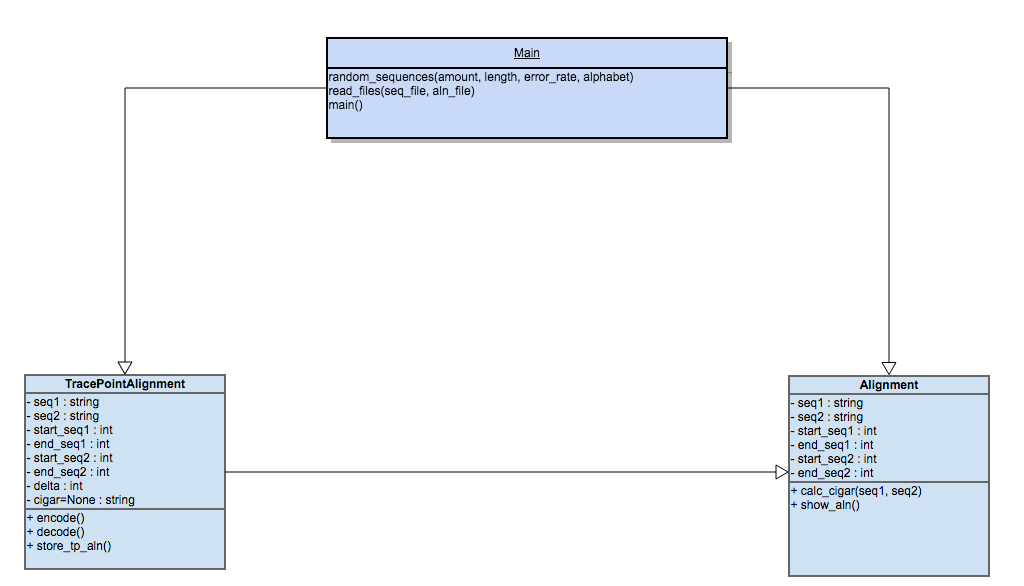
\includegraphics[width=\textwidth]{images/UML}
	\caption{UML-Diagramm}
\end{figure}

\clearpage

\section{Funktionalit�t}

\begin{algorithm}[h]
	\caption{Computation of Trace Points from a given CIGAR-String}
	\label{encode}
	\noindent\begin{tabular}{@{}l@{~}l}
		\textbf{Input}:
		&$seq1, seq2, start\_seq1, end\_seq1, start\_seq2, \Delta, cigar$ mit \\
		&$\Size{seq1}, \Size{seq2}, \Size{cigar} > 0$;\\
		&$start\_seq1, start\_seq2 \geq 0$;\\
		&$start\_seq1 < end\_seq1$ und\\
		&$\Delta > 0$\\
		\textbf{Output}:&Array $TP$ of Trace Points
	\end{tabular}
	\medskip
	\begin{algorithmic}[1]
		\Function{\textit{encode}}{$seq1, seq2, start\_seq1, end\_seq1, start\_seq2, \Delta, cigar$}
		\State \Assign{itv\_size}{MAX(1, \Roundup{start\_seq1/\Delta})}
		\State \Assign{itv\_count}{MIN(\Roundup{\Size{seq1}/\Delta}, \Roundup{\Size{seq2}/\Delta})}
		\For{\Assign{i}{0} \Upto \(\Size{itv\_count}\)} \\
		\Assign{\indent itv[i]}{
			\begin{cases}
				start\_seq1, itv\_size \cdot \Delta - 1&\text{ if } i = 0\\
				(itv\_size + i - 1) \cdot \Delta, (itv\_size + i) \cdot \Delta - 1&\text{ if } 0 < i < \Size{itv\_count}\\
				(itv\_size + i - 1) \cdot \Delta, end\_seq1 - 1&\text{ else.}
			\end{cases}}
			\EndFor
			\State \Assign{count1, count2, count3}{0}
			\State \Assign{TP}{\text{Array for Trace Points}}
			\For{\text{each $(cig\_count, cig\_symbol)$ in cigar}}
			\For{\Assign{i}{0} \Upto \(cig\_count\)}
			\If{cig\_symbol = 'I'}
			\State increment $count1$
			\ElsIf{cig\_symbol = 'D'}
			\State increment $count2$
			\Else
			\State increment $count1, count2$
			\EndIf
			
			\If{count1 = intervals[count3][1] + 1 \textbf{and} count1 $\neq \Size{seq1}$}
			\State append (count2 - 1 + start\_seq2) to $TP$
			\EndIf
			\If{count $\neq \Size{itv} - 1$}
			\State increment $count3$
			\EndIf
			\EndFor
			\EndFor
			\State \Return $TP$
			\EndFunction
		\end{algorithmic}
	\end{algorithm}

\FloatBarrier
\subsection{Informationsverlust bei 'encode()'}
Die encode-Funktion extrahiert aus dem gegebenen CIGAR-String die Trace Points, welche dann zusammen mit dem $\Delta$-Wert und den Start- und Endpositionen der Sequenzabschnitte gespeichert werden. Hierbei geht die Information, wie die jeweiligen Intervalle zwischen den Trace Points zu den komplement�ren Intervallen in der Ursprungssequenz aligniert werden, verloren.
F�r die R�ckgewinnung dieser Information muss in der 'decode()'-Funktion zun�chst ein neues Alignment der jeweiligen Intervall-Paare errechnet werden.
%\FloatBarrier

\begin{algorithm}[h]
	\caption{Computation of a CIGAR-String from a given Trace Point Array}
	\label{decode}
	\noindent\begin{tabular}{@{}l@{~}l}
		\textbf{Input}:
		&$seq1, seq2, \Delta, TP$ mit\\
		&$\Size{seq1}, \Size{seq2}, \Delta, \Size{TP} > 0$\\
		\textbf{Output}:&CIGAR-String
	\end{tabular}
	\medskip
	\begin{algorithmic}[1]
		\Function{\textit{decode}}{$seq1, seq2, \Delta, TP$}
		\State \Assign{cig}{\text{empty String}}
		\For{\Assign{i}{0} \Upto \(\Size{TP}\)}
		\If{i = 0}
		\State append \textbf{cigar}($seq1[0...\Delta], seq2[0...TP[i] + 1]$) to $cig$
		\ElsIf{i = \Size{TP} - 1}
		\State append \textbf{cigar}($seq1[i \cdot \Delta...\Size{seq1}], seq2[TP[i - 1] + 1...\Size{seq2}]$) to $cig$
		\Else
		\State \begin{tabular}{rll}
			append \textbf{cigar}&($seq1[i \cdot \Delta...(i + 1) \cdot \Delta],$&\\
			&$seq2[TP[i - 1] + 1]...TP[i] + 1$)& to $cig$
		\end{tabular}
		
		\EndIf
		\EndFor
		\State \Assign{cig}{\textbf{combine}(cig)}
		\State \Return cig
		\EndFunction\\
		
		\Function{\textit{combine}}{$cigar$}
		\State \Assign{cig}{\text{empty String}}
		\State \Assign{tmp}{0}
		\For{\text{each $(cig\_count, cig\_symbol)$ in cigar}}
		\State \Assign{tmp}{tmp + previous\_cig\_count}
		\If{cig\_symbol = previous\_cig\_symbol}
		\If{\text{not last element in cigar}}
		\State \Assign{tmp}{0}
		\EndIf
		\EndIf
		\If{\text{last element in cigar}}
		\State \text{append $(tmp + cig\_count, cig\_symbol)$ to cig}
		\EndIf
		\EndFor
		\State \Return cig
		\EndFunction
	\end{algorithmic}
\end{algorithm}